\documentclass[a4paper,12pt]{article}

\usepackage{polyglossia}
\setdefaultlanguage{english}
\setotherlanguage{russian}
\usepackage[shortcuts]{extdash}

\usepackage{adjustbox}

\usepackage{fontspec}
\usepackage{xunicode}
\usepackage{xltxtra}
\usepackage{libertine} 
\usepackage{indentfirst}
\usepackage{listings}
\usepackage{color}
\definecolor{codegray}{rgb}{0.5,0.5,0.5}
%\setmainfont{Garamond}

\usepackage[colorlinks,allcolors=black]{hyperref}

\usepackage{soul} 
\usepackage{csvsimple}

% Библиография
\usepackage[autostyle]{csquotes}

\usepackage[backend=biber,style=authoryear]{biblatex}
\addbibresource{mybiblio.bib}

%\DeclareBibliographyCategory{ignore}

% Библиографию в оглавление
\usepackage[nottoc]{tocbibind}

%% Перенос знаков в формулах (по Львовскому)
\newcommand*{\hm}[1]{#1\nobreak\discretionary{}
{\hbox{$\mathsurround=0pt #1$}}{}}

%%% Работа с картинками
\usepackage{graphicx}  % Для вставки рисунков
%\graphicspath{{images/}{images2/}}  % папки с картинками
\setlength\fboxsep{3pt} % Отступ рамки \fbox{} от рисунка
\setlength\fboxrule{1pt} % Толщина линий рамки \fbox{}
\usepackage{wrapfig} % Обтекание рисунков текстом

%%% Работа с таблицами
\usepackage{array,tabularx,tabulary,booktabs} 
\usepackage{longtable} 
\usepackage{multicol}
\usepackage{multirow}
\usepackage{xcolor}
\renewcommand\arraystretch{1.1}

\usepackage{tikz-dependency}

\usepackage{caption}	

\usepackage{setspace} % Интерлиньяж


\usepackage{titlesec}
\titleformat{\chapter}[display]
{\normalfont\Large\bfseries\flushleft}{\chaptertitlename\ \thechapter}{0.2em}{\LARGE}
\titleformat{\section}
{\normalfont\large\bfseries\flushleft}{\thesection}{0.5em}{}
\titleformat{\subsection}
{\normalfont\normalsize\bfseries\flushleft}{\thesubsection}{0.5em}{}
\titlespacing*{\chapter}{0pt}{0em}{1em}
\titlespacing*{\section}{0pt}{1.5em}{0.5em}
\titlespacing*{\subsection}{0pt}{1em}{0.25em}

% Лингвистика
\usepackage{gb4e}
\usepackage{qtree}


\author{Михаил Воронов}
\title{Дипломная работа}
\date{\today}

\begin{document} % конец преамбулы, начало документа

\newpage
\thispagestyle{empty}
\begin{center}
    \textbf{Правительство Российской Федерации \\
        Федеральное государственное автономное образовательное \\
        учреждение высшего образования}
    \vspace{1cm}

    \textbf{Национальный исследовательский университет \\ <<Высшая школа экономики>>}
\end{center}

\vspace{1cm}
\begin{flushright}
    \noindent
    Факультет гуманитарных наук \\
    Образовательная программа \\
    <<Фундаментальная и компьютерная лингвистика>>
\end{flushright}

\begin{center}
    Воронов Михаил Кириллович \\
    \vspace{2ex}
    \textbf{Программная библиотека для лингвистической типологии на языке Python} \\
    \textit{Python Library for Linguistic Typology}\\
    \vspace{3ex}
    Выпускная квалификационная работа студента 4 курса бакалавриата 
\end{center}
\vspace{3ex}
\begin{tabular}{p{0.4\linewidth}p{0.45\linewidth}}
    Академический~руководитель образовательной программы & Научный руководитель \\
    канд.~филологических наук, доц. & канд.~филологических наук, доц.\\
    Ю.А.Ландер & Б.В.Орехов \\
    & \\ 
    4 июня 2019 г.
\end{tabular}

\begin{center}
    Москва 2019
\end{center}

\newpage

\setcounter{tocdepth}{2}
\tableofcontents

\newpage
\section{Introduction}
There are multiple programming tools used by linguists. Such tools as PRAAT and ELAN have become essential instruments in phonological research~\parencite{praat}~\parencite{elan}.

PRAAT is written in C and C++ programming languages and ELAN is written in Java. However, majority of other linguistic tools is written in Python~\parencite{python}.

There are reasons for this.
\begin{itemize}
 \item Python concentrates on simplicity and readability of code~\parencite{zen}.
 \item Python provides good support for Unicode which is crucial for linguistics~\parencite{unicode}~\parencite{python}.
 \item There is a wide variety of Python libraries for scientific research such as SciPy or Pandas~\parencite{scipy}~\parencite{pandas}.
 \item Multiple linguistic tools (see below) are already written for Python. It provides good community support.
\end{itemize}

Many Python tools concentrate on natural language processing (e.g. NLTK \parencite{NLTK}). There are also some libraries that are there to assist linguistic research.

A good example of such package is LingPy~\parencite{List2017i}. It provides multiple calculation and visualization algorithms for historical linguistics.

Another example of this kind of libraries is LingCorpora~\parencite{alexey}. It allows to perform queries in multiple online text corpora. It is in active development at the moment and already supports more than 25 corpora.

However, it seems that Python tools that allow to work with linguistic online databases do not exist.

Most of such databases are stored in Cross-Linguistic Linked Data format \parencite{CLLD}. This specification also provides framework~\parencite{RobertForkel2019} that allows creating CLLD apps. However, it does not provide user-friendly API for the stored data and cannot access databases from remote repositories.

There is a tool for Glottolog~\parencite{HaraldHammarstrom2019} that provides an API and console application for Glottolog~\parencite{Robert2Forkel2019}. However, this tool requires a local copy of Glottolog data that takes more than 700 megabytes of storage. It is too much for an average laptop and it takes some time to download even with decent wired Internet connection.

Also, there seems to be no Python tools for linguistic interactive mapping and researchers have to use libraries such as Folium~\parencite{folium} which is a general tool for interactive mapping and is not designed for linguistic maps specifically.

So, the first gap that my package attempts to cover is lack of Python tools that provide an interface for online linguistic databases. The second gap is lack of Python tools designed for linguistic interactive mapping. The combination of these features may be useful for typological research that rely on data from linguistic databases and require geographical visualization. There is a good example of such research \parencite{Blasieaav3218}. It relies on data from PHOIBLE \parencite{phoible} and Autotyp \parencite{autotyp} databases and uses geographical maps.

There is a package for the R programming language called 'lingtypology' \parencite{GeorgeMoroz2018}. It provides an API for linguistic databases, a tool to work with Glottolog data and a tool to create interactive linguistic maps. My package was inspired by this R library and I consider it to be its counterpart for Python. Therefore my package is also called 'lingtypology'. The Python counterpart is necessary because now Python is de-facto standard language for linguistic tools and a project is more likely to receive extra support from community. Among other reasons there are: better readability of Python code than readability of R code, lower memory consumption by Python interpreter and more flexibility because, unlike R which is mostly restricted to scientific tools, Python is a versatile language. Therefore, creating a Python counterpart will allow to use the package within other linguistic tools and implement it into websites. Due to these reasons, Python counterpart of the R package seems to be necessary.

One of the main purposes of my package is to provide a tool for easy reproducibility. Lack of reprodicibility is a severe problem in any area of science. There is an article on this problem that states that there `are many technical reasons why experimental results, particularly in cancer research, cannot be reproduced, including unrecognized variables in the complex experimental model, 
poor documentation of procedures, selective reporting of the most-positive findings, 
misinterpretation of technical noise as biological signal and, in the most extreme 
cases, fabrication of data.`~\parencite{Pusztai2013}

Unfortunately, these problems also apply to typological studies. LingTypology presents an interface for linguistic databases and, as a computer program, the result will be always the same. To guarantee reproducibility of research made using LingTypology, it is distributed under GNU GPL License and therefore the whole source code is open so that anybody could read it and make sure it works as expected.

Also, usually researchers manually find the data from multiple linguistic research. With my package it is possible to reproduce such research very quickly.

Reproducibility is a very important thing in scientific research and LingTypology aims to assist researchers to reproduce other studies and make their own studies reproducible.

In the following chapters, I will describe technical aspects of LingTypology, provide documentation and several small studies to demonstrate its usability.

\newpage


\section{Project Description}
In this section I will provide description for \texttt{lingtypology}. To avoid repetition I will not include documentation into this section, it is present in Chapter~3~'Usage'.

\subsection{General}
\texttt{lingtypology} is written in the Python programming language, version 3.7~\parencite{python}. It also supports versions 3.5 and 3.6. It is planned to keep maintaining all the versions of Python that are supported except for 2.7 branch. It is not supported due to maintenance difficulty and its coming end of life in early 2020.

This project uses \texttt{git} distributed version control system. The source code of the project is stored in the remote repository~\parencite{MichaelVoronov2019}.

\subsection{Dependencies}
\texttt{lingtypology} package requires a number of additional libraries.
\begin{itemize}
\begin{samepage}
  \item Folium and Branca~\parencite{folium}. Folium is a Python wrapper for \texttt{leaflet} library for JavaScript~\parencite{leaflet}. Branca is the additional package for Folium that allows editing HTML code of the maps while Folium works with JavaScript only. 
  \item Pandas~\parencite{pandas}. Pandas introduces dataframes in Python.
  \item pyglottolog~\parencite{Robert2Forkel2019}. \texttt{pyglottolog} application is used to extract necessary data from Glottolog.
  \item matplotlib~\parencite{matplotlib}. Matplotlib is a tool for creating plots.
  \item jinja2. A template engine.
  \item colour. A library for colors.
\end{samepage}
\end{itemize}

\subsection{Package}
\texttt{lingtypology} package consists of different modules and data files.

\subsubsection{Modules}
\begin{itemize}
\begin{samepage}
 \item \texttt{\_\_init.py\_\_} contains imports and version.
 \item \texttt{maps.py} is the module for linguistic interactive mapping.
 \item \texttt{glottolog.py} contains a number of useful functions for Glottolog.
 \item \texttt{db\_apis.py} contains API for multiple online databases.
\end{samepage}
\end{itemize}
\subsubsection{Data Files}
\begin{itemize}
\begin{samepage}
 \item \texttt{legend.html} HTML-template for map legends and title. Based on the code from the Internet~\parencite{legend}.
 \item \texttt{language\_elevation\_mapping.json} data on elevation for each language from Glottolog.
 \item \texttt{autotyp\_lang\_mapping.json} mapping from language IDs from Autotyp to languages from Glottolog. Taken from the R counterpart under the rule of GNU GPL license~\parencite{GeorgeMoroz2018}.
 \item CSV file that starts with \texttt{glottolog-languoids} contains some of Glottolog data. It is generated with \texttt{pyglottolog} application with \texttt{glottolog --repos=glottolog languoids} command.
 \item JSON file that starts with \texttt{glottolog-languoids} contains metadata for the CSV file above.
\end{samepage}
\end{itemize}


\subsection{Interactive Maps}
In this subsection I will describe the obstacles overcome for creation of \texttt{lingtypology.maps} module.

\subsubsection{General}
\texttt{lingtypology.maps} contains the \texttt{LingMap} object. This object has attributes and methods that allow to render interactive maps. This object stores the data that a user wants to be rendered and when \texttt{create\_map} method is called all the data is processed and passed into \texttt{folium.map} object. Then it can be rendered as \texttt{HTML}.

For example, method \texttt{add\_overlapping\_features} applies different colors from \texttt{colors} atrribute to each feature, finds out the proper size of markers based on the amount of features for each language, creates 
\texttt{folium.CircleMarker} objects, adds popups and tooltips to the markers if necessary and then adds the markers to the map.

Also, \texttt{lingtypology.maps} contain several supplementary functions.

Full description of the functions and the \texttt{LingMap} class can be found in Chapter~3.

\subsubsection{Elevation Data}
\texttt{lingtypology} provides elevation data for each language in Glottolog (as of version 3.4). The source of this data is SRTM dataset~\parencite{SRTM}.
It was processed using locally run Open Elevation API server~\parencite{OpenElevation}.

Open Elevation API is an API that allows to get elevation data for give coordinates from the given GeoTIFF dataset. By default it uses SRTM dataset. Open Elevation API is accessible online. However, it was not able to handle the request that I sent (around 8000 coordinates). Open Elevation is open-source, so I was able to deploy it locally and run it with the SRTM-data. Then I sent my request to my locally deployed Open Elevation API server and got the result for the coordinates from the Glottolog dataset.

After that, I mapped the elevation data to the languages from Glottolog \parencite[language\_elevation\_mapping.json]{MichaelVoronov2019}.

\subsubsection{Legend}
Folium does not provide API to create a legend. Nevertheless, Lingtypology has a legend. It is created automatically based on the data that user passes to lingtypology.

The template for the legend is based on the HTML code from here~\parencite{legend}.

\subsubsection{Strokes}
The default appearance of standard \texttt{folium.CircleMarker} objects does not fit the needs of the package due to the behaviour of strokes. Compare pictures 1 and 2.

In the first picture strokes appear after each individual marker (the default behaviour of \texttt{folium}).
In the second picture strokes appear after groups of markers. This bahaviour is impossible to achive using \texttt{folium.CircleMarker} objects by default. Therefore, instead of rendering one marker with stroke, \texttt{lingtypology} renders two markers: a marker without stroke and a black marker that 115\% larger. Markers are not added to the map right away. They are rendered in the proper order:
\begin{enumerate}
 \item Draw all black background markers.
 \item Draw normal markers.
\end{enumerate}

The way markers are rendered in the second figure is the default behaviour of \texttt{lingtypology}. However, the option to use the standard behaviour of \texttt{foilum} is present as well.

Both figures were generated using \texttt{lingtypology}. Listings are in the Appendix ('Listing 2' and 'Listing 1').
\bigskip

\noindent
\begin{minipage}{\textwidth}
\captionof{figure}{Default Folium strokes}
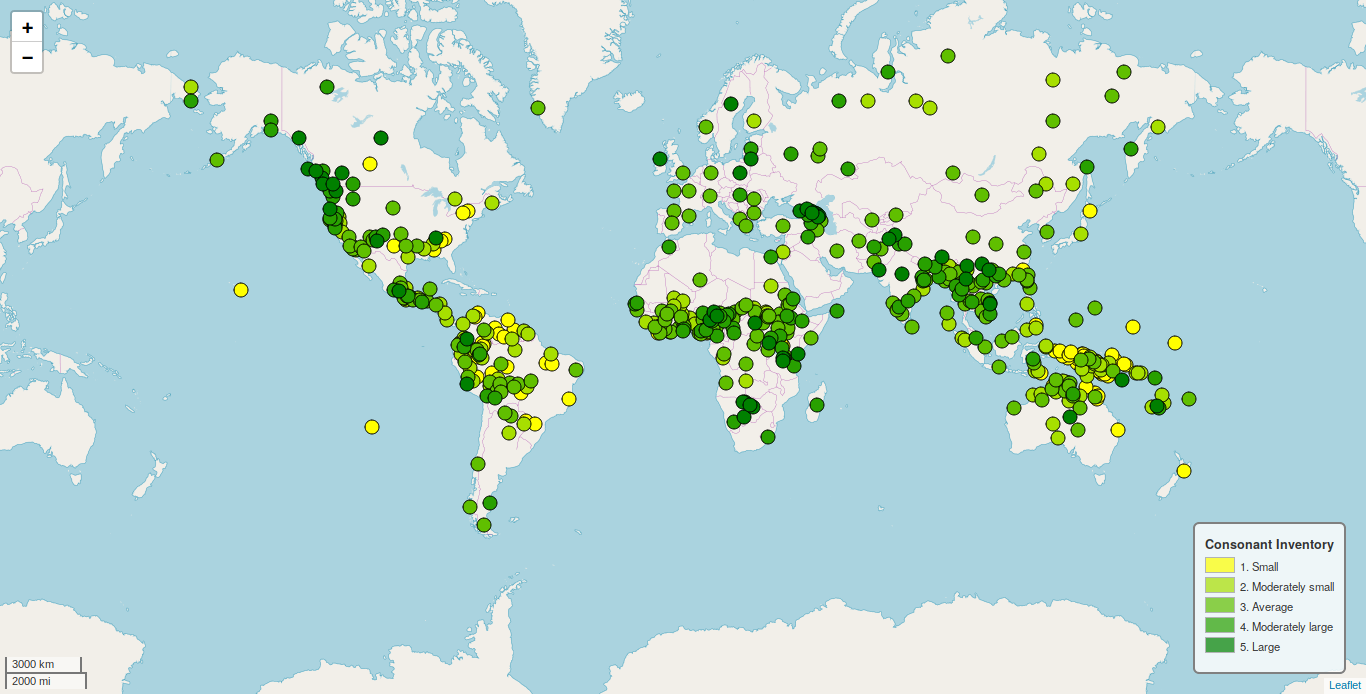
\includegraphics[width=\textwidth]{images/FoliumStrokeAppearance.png}
\bigskip
\end{minipage}

\noindent
\begin{minipage}{\textwidth}
\captionof{figure}{Default Lingtypology strokes}
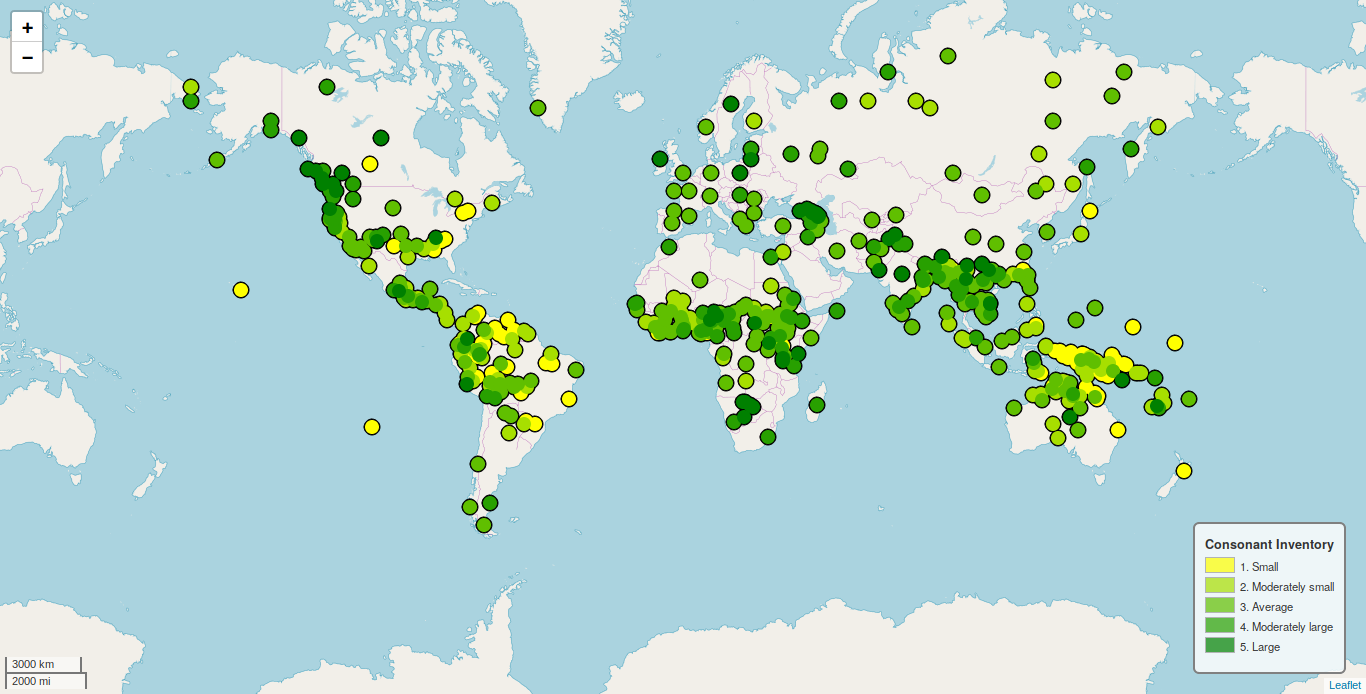
\includegraphics[width=\textwidth]{images/LingtypologyStrokeAppearance.png}
\bigskip
\end{minipage}

\subsubsection{Minicharts}

I had a feature request to add functionality to draw minicharts instead of markers in the map.

Due to the fact that neither \texttt{folium} nor \texttt{folium.plugins} does not provide such functionality and I did not find a Leaflet plugin with such functionality, minicharts are rendered as SVG with Matplotlib~\parencite{matplotlib}.

Matplotilib does provide functionality to render plots as SVG images and save them as plain text files. Nevertheless, it does not provide documentation for methods that allow to get SVG as Python type \texttt{str}. Therefore, the plots rendered as SVG have to be caught with \texttt{io.StringIO} object from standard Python library.

Object \texttt{folium.Marker} allows passing HTML elements that define their appearance. However, it is not possible to pass the SVG as is: if there are newline symbols, the HTML file of the map will be broken. Therefore, all such symbols have to be removed from the SVG string.

Due to lack of unified API for different charts in Matplotlib, the number of available minicharts is limited. At the moment only pie-charts and bar-charts are supported.

During this research I received a request from one of the Folium developers to add an example of minicharts usage to the Folium gallery. My example is available in the `examples` directory of the Folium repository~\parencite{folium}.

\subsubsection{PNG}

Foium does not provide official support for rendering maps as PNG. Nevertheless, I found undocumented API that allows it (\texttt{folium.Map.\_to\_png} method).

It was implemented into Lingtypology. However, this method requires additional application (Geckodriver) which is not included into main repositories of some popular operating systems (Windows, macOS, Debian GNU/Linux, OpenSUSE etc.) and requires additional efforts to install. Due to this fact, this functionality of Lingtypology is marked as experimental until another way to implement is found. Also, this functionality requires additional Python dependency: \texttt{selenium}. It is used to render HTML as PNG.

\subsection{Glottolog}

\texttt{lingtypology} uses Glottolog data at its core. Therefore, accessing it online each time would significantly slow down the package. Glottolog data necessary for the package is included in the package.

However, Glottolog data is updated continually. I update included Glottolog data with each new release of \texttt{lingtypology}. If user requires newer version of the data before new release, I provide the instruction how to update it manually.

\texttt{lingtypology.glottolog} provides multiple functions to work with Glottolog data. Usage information may be found in Chapter 3.

\subsection{Databases API}

\texttt{lingtypology} provides API for the following lingustic databases:
\begin{itemize}
\begin{samepage}
 \item WALS~\parencite{wals}.
 \item Autotyp~\parencite{autotyp}.
 \item AfBo~\parencite{afbo}.
 \item SAILS~\parencite{sails}.
 \item PHOIBLE~\parencite{phoible}
\end{samepage}
\end{itemize}

\subsubsection{General}
Databases usually can be retrieved in CSV format. They are read into \texttt{pandas.DataFrame}, processed and returned to user in easy to read and use format.

\texttt{lingtypology.db\_apis} contains classes for each database. The module attemts to provide a unified API for all datasets, so there are methods that work the same way for all the databases.

The moment when the database is downloaded depends on the database. In some cases the data is received right after the initialization of the respective class, in other cases the data is downloaded when \texttt{get\_df} method is called.

If the data in the database is divided into different pages, tables etc., \texttt{lingtypology} is able to process and merge several of them.

\subsubsection{WALS}
WALS: 'The World Atlas of Language Structures (WALS) is a large database of structural (phonological, grammatical, lexical) properties of languages gathered from descriptive materials (such as reference grammars) by a team of 55 authors.'~\parencite{wals}. The data from wals is retrieved from multiple web-pages that contain data for each chapter when \texttt{get\_df} method is called.

\subsubsection{Autotyp}
Autotyp is database that contains of multiple modules. Each module represents a grammatical feature (e.g. Agreeement), it contains information on this feature for various languages~\parencite{autotyp}. The data is downloaded when \texttt{get\_df} method is called.

\subsubsection{AfBo}
AfBo: A world-wide survey of affix borrowing~\parencite{afbo}. AfBo contains information about borrewed affixes in different languages. It provides data in ZIP archive with CSV files. The data is downloaded with initialization of the class.

\subsubsection{SAILS}
`The South American Indigenous Language Structures (SAILS) is a large database of grammatical properties of languages gathered from descriptive materials (such as reference grammars)`~\parencite{sails}. Like in the case of AfBo, SAILS data is available in ZIP archive. The data is downloaded with initialization of the class.

\subsubsection{PHOIBLE}
`PHOIBLE is a repository of cross-linguistic phonological inventory data, which have been extracted from source documents and tertiary databases and compiled into a single searchable convenience sample.`~\parencite{phoible}.
Unlike other databases supported by Lingtypology, PHOIBLE is not a unified dataset. It contains data of the following datasets: UPSID, SPA, AA, PH, GM, RA, SAPHON.

\newpage

\section{Usage}
In this part I will provide full guide for \texttt{lingtypology} package. It is divided into four parts: Installation, Interactive Maps, Glottolog functions and the API for databases.

\subsection{Installation}
The package is uploaded to PyPI software repository, therefore it can be installed with the \texttt{pip} utility with the following command:

\texttt{pip3 install lingtypology --user}

\subsection{Interactive Maps}
Interactive maps can be created with \texttt{lingtypology.maps} module.

\subsubsection{LingMap Class}

\textit{class} lingtypology.\textbf{LingMap} \textit{(languages=[], glottocode=False)}

Bases: \textit{object}

\textbf{Parameters}:
\begin{itemize}
\begin{samepage}
 \item \textbf{languages}: \textit{list} or \textit{pandas.Series} of strings, default \textit{[]}.

 A list of languages. The language names should correspond to their names from Glottolog unless you use \textit{add\_custom\_coordinates} method.
 
 Instead of language names you could use Glottocodes (language ID in Glottolog). In this case you need to set \textit{glottocode} parameter to true.
 
 \item \textbf{glottocode}: \textit{bool}, default \textit{False}.
 
 Whether to treat \textit{languages} as Glottocodes.
 
\end{samepage}
\end{itemize}

\textbf{Attributes}:
\begin{itemize}
 \item \textbf{tiles}: \textit{str}, default \textit{'OpenStreetMap'}
 
 Tiles for the map. You can use one of these tiles (list of tiles is borrowed from the Folium Documentation~\parencite{foliumDocs}):
 \begin{itemize}
 \item “OpenStreetMap”
 \item “Mapbox Bright” (Limited levels of zoom for free tiles)
 \item “Mapbox Control Room” (Limited levels of zoom for free tiles)
 \item “Stamen” (Terrain, Toner, and Watercolor)
 \item “Cloudmade” (Must pass API key)
 \item “Mapbox” (Must pass API key)
 \item “CartoDB” (positron and dark\_matter)
 \item or pass the custum URL.
 \end{itemize}
 \item \textbf{start\_location}: \textit{(float, float)} or \textit{str}, default \textit{(0, 0)}
 
 Coordinates of the start location for the map \textit{(latitude, longitude)} or a text shortcut. List of available shortcuts: \textit{"Central Europe", "Caucasus", "Australia \& Oceania", "Papua New Guinea", "Africa", "Asia", "North America", "Central America", "South America"}.
 \item \textbf{start\_zoom}: \textit{int}, default \textit{2}
 
 Initial zoom level. Bypassed if you are using a shortcut \textit{start\_location}.
 
 \item \textbf{control\_scale}: \textit{bool}, default \textit{True}
 
 Whether to add control scale.

 \item \textbf{prefer\_canvas}: \textit{bool}, default \textit{False}

 Use canvas instead of SVG. If set to True, the map may be more responsive in case you have a lot of markers.
 
 \item \textbf{base\_map}: \textit{folium.Map}, default \textit{None}
 
 In case you want to draw something on particular \textit{folium.Map}.
    
 \item \textbf{title}: \textit{str}, default \textit{None}
 
 You can add a title to the map.
 
 \item \textbf{legend}: \textit{bool}, default \textit{True}
 
 Whether to add legend for features (\textit{add\_features} method).
 
 \item \textbf{stroke\_legend}: \textit{bool}, default \textit{True}.

 Whether to add legend for stroke features (\textit{add\_stroke\_features} method)

 \item \textbf{legend\_title}: \textit{str}, default \textit{'Legend'}
 
 Legend title.
 
 \item \textbf{stroke\_legend\_title}: \textit{str}, default \textit{'Legend'}
 
 Stroke legend title.
 
 \item \textbf{legend\_position}: \textit{str}, default \textit{'bottomright'}
 
 Legend position. Available values: 'right', 'left', 'top', 'bottom', 'bottomright', 'bottomleft', 'topright', 'topleft'.

 \item \textbf{stroke\_legend\_position}: \textit{str}, default \textit{'bottomleft'}
 
 Stroke legend position. Available values: 'right', 'left', 'top', 'bottom', 'bottomright', 'bottomleft', 'topright', 'topleft'.
 
 \item \textbf{colors}: \textit{list} of html codes for colors (\textit{str}).
 
 Colors that represent features. You can either use the 20 default colors or set yours.
 
 \item \textbf{stroke\_colors}: \textit{list} of html codes for colors (\textit{str})
 
 Colors that represent additional (stroke) features.

 \item \textbf{shapes}: \textit{list} of characters (\textit{str})
 
 If you use shapes instead of colors, you can either use the default shapes or set yours. Shapes are Unicode symbols.

 \item \textbf{stroked}: \textit{bool}, default \textit{True}
 
 Whether to add stroke to markers.

 \item \textbf{unstroked}: \textit{bool}, default \textit{True}
 
 If set to True, circle marker will merge if you zoom out without stroke between them. It multiplies the number of markers by 2. For better performance set it to False. More information and examples in Chapter 2, Paragraph 4.4.
 
 \item \textbf{languages\_in\_popups}: \textit{bool}, default \textit{True}
 
 Whether to show links to Glottolog website in popups.
 
 \item \textbf{control}: \textit{bool}, default \textit{False}
 
 Whether to add LayerControls and group by features.

 \item \textbf{stroke\_control}: \textit{bool}, default \textit{False}
 
 Whether to add LayerControls and group by stroke features.
 
 \item \textbf{control\_position}: \textit{str}, default \textit{'topright'}
 
 Position of LayerControls. May be ‘topleft’, ‘topright’, ‘bottomleft’ or ‘bottomright’.

 \item \textbf{colormap\_colors}: \textit{tuple}, default \textit{('white', 'green')}
 
 Colors for the colormap.

\end{itemize}

\textbf{Methods}:

\begin{itemize}

 \item \textbf{add\_custom\_coordinates} \textit{(custom\_coordinates)}

 Set custom coordinates. By default cooordinates for the languages are taken from the Glottolog database. If you have coordinates and want to use them, use this function.
 
 It could be useful if you are using data from a dataset which provides coordinates and you do not need to rely on the Glottolog data.
        
 \textbf{Parameter} custom\_coordinates: \textit{list} of custom\_coordinates (\textit{tuples})
 
 Length of the list should equal to length of languages.

 \item \textbf{add\_features}\textit{(features, radius=7, opacity=1, numeric=False, control=False, use\_shapes=False)}
 
 Add features to the map.
 
 \textbf{Parameters}:
 \begin{itemize}
 \item \textbf{features}: \textit{list}
 
 List of features. Amount of features should be equal to the amount of languages.
 By default, if you add features, a legend will appear. To shut it down set \textit{legend} attribute to \textit{False}.
 To change the title of the legend use \textit{legend\_title} attribute.
 To change legend position use use \textit{legend\_position} attribute.
 
 \item \textbf{radius}: \textit{int}, default \textit{7}
 
 Marker radius.
 
 \item \textbf{numeric}: \textit{bool}, default \textit{False}
  
  Whether to assign different color to each feature (\textit{False}), or to assign a color from colormap (\textit{True}).
  You can set it to True only in case your features are numeric and stroke features are not given.
  To change the default colors of the color scale use \textit{colormap\_colors} attribute.
  
  \item \textbf{control}: \textit{bool}, default \textit{False}

  Whether to add LayerControls to the map.
  It allows interactive turning on/off given features.

  \item \textbf{use\_shapes}: \textit{bool}, default \textit{False}

  Whether to use shapes instead of colors. This option allows to represent features as shapes.
  Shapes are Unicode charaters. You can replace or add to default symbols by changing \textit{shapes} attribute.
  If colors are not a viable option for you, you can set this option to True.
  
 \end{itemize}
 
 \item \textbf{add\_stroke\_features}\textit{(features, radius=12, opacity=1, numeric=False, control=False)}:
 
 Add additional set of features that look like strokes around markers.
 
 \begin{itemize}
 \item \textbf{features}: \textit{list}
 
 List of additional features. Amount of features should be equal to the amount of languages.
 By default, if you add stroke features, a legend will appear. To shut it down set \textit{stroke_legend} attribute to \textit{False}.
 To change the title of the legend use \textit{stroke\_legend\_title} attribute.
 To change legend position use use \textit{stroke\_legend\_position} attribute.
 
 \item \textbf{radius}: \textit{int}, default \textit{12}
 
 Marker radius. Note that this radius is absolute as well.
 
 \item \textbf{control}: \textit{bool}, default \textit{False}
  
  Whether to add LayerControls to the map.
  It allows interactive turning on/off given stroke features.

 \end{itemize}
 
 \item \textbf{add\_overlapping\_features} \textit{(features, radius=7, radius\_increment=4, mapping=None)}:
 
 Add overlapping features.
 For example, if you want to draw on map whether language 'is ergative', 'is slavic', 'is spoken in Russia'.
 It will draw several markers of different size for each feature.
 
 \textbf{Parameters}:
 
 \begin{itemize}
 \item \textbf{features}: \textit{list} of lists
 
 List of features. Amount of features should be equal to the amount of languages.
 
 \item \textbf{radius}: \textit{int}, default 7
 
 Radius of the smallest circle.
 
 \item \textbf {radius\_increment}: \textit{int}, default \textit{4}
 
 Step by which the size of the marker for each feature will be incremented.
 
 \item \textbf {mapping}: \textit{dict}, default \textit{None}
 
 Mapping for the legend.
 
 \end{itemize}
 
 \item \textbf{add\_minicharts} \textit{(*minicharts, typ='pie', size=0.6, names=None, textprops=None, labels=False, colors=[], startangle=90)}:
 
 Create minicharts using Maplotlib.
 
 \textbf{Parameters}:
 
 \begin{itemize}
 \item \textbf{*minicharts}: list-like objects
 
 Data for minicharts. Two list-like objects.
 
 \item \textbf{typ}: \textit{str}, default \textit{pie}
 
 Type of the minicharts. Either \textit{pie} or \textit{bar}.
 
 \item \textbf{size}: \textit{float}
 
 Size of the minicharts.
 
 \item \textbf{texprops}: \textit{dict}, default \textit{None}
 
 Textprops for Matplotlib.
 
 \item \textbf{labels}: \textit{bool}, default \textit{False}
 
 Whether to display labels.
 
 \item \textbf{colors}: \textit{list}, default \textit{[]}
 
 Minicharts colors.
 
 \item \textbf{startange}: \textit{int}, default \textit{90}
 
 Start angle of pie-charts (pie-charts only).
 
 \end{itemize}
 
 \item \textbf{add\_heatmap}: \textit{(heatmap=[])}
    
    Add heatmap.
    
    \textbf{Parameter} heatmap: list-like object with tuples
    
    Coordinates for the heatmap. To create a heatmap-only map, do not pass any languages.

 \item \textbf{add\_popups} \textit{(popups, parse\_html=False)}
    
    Add popups to markers.
    
    \textbf{Parameters}:
    \begin{itemize}
     \item \textbf{popups}: \textit{list} of strings
       List of popups. Length of the list should equal to length of languages.
     \item \textbf{parse\_html}: \textit{bool}, default \textit{False}
       By default (\textit{False}) you can add HTML elements.
       If you need to add full HTML pages to popups, you need to set the option to \textit{True}.
    \end{itemize}
    
 \item \textbf{add\_tooltips} \textit{(tooltips)}:
 
    Add tooltips to markers.
    
    \textbf{Parameter} tooltips: \textit{list} of strings
    
    List of tooltips. Length of the list should equal to length of languages.

 \item \textbf{add\_minimap} \textit{(position='bottomleft', width=150, height=150, collapsed\_width=25, collapsed\_height=25, zoom\_animation=True)}
 
 Add minimap.

 \textbf{Parameters}:
 \begin{itemize}
  \item \textbf{position}: \textit{str}, default \textit{'bottomleft'}
  \item \textbf{width} and \textbf{height}: \textit{int}, default \textit{150}
  \item \textbf{collapsed\_width} and \textbf{collapsed\_height}: \textit{int}, default \textit{25}
  \item \textbf{zoom\_animation}: \textit{bool}, default \textit{True}
  
  You can disable zoom animation for better performance.
 
 \end{itemize}
 
 \item \textbf{add\_line} and \textbf{add\_rectangle} \textit{(locations, tooltip='', popup='', color='black')}
 
 \textbf{Parameters}:
 \begin{itemize}
  \item \textbf{locations}: list-like object of tuples
  
  Coordinates necessary ro draw the figure.
  
  \item \textbf{tooltip}: \textit{str}, default ''
  
  Tooltip for the figure.
  
  \item \textbf{popup}: \textit{str}, default ''
  
  Popup for the figure.
  
  \item \textbf{color}: \textbf{str}, default 'black'
  
  Color of the figure.
  
 \end{itemize}

 
 \item \textbf{create\_map} \textit{()}
 
 Create the map. To display the map in Jupyter Notebook, use this function.
 
 \textbf{Returns} folium.Map
 
 \item \textbf{render}\textit{()}
 
 \textbf{Returns} the HTML code as \textit{str}. It might be useful in case you want to implement it into a website.
 
 \item \textbf{save} \textit{(path)}
 
 Save the map as HTML. It is useful when you need to include a map into a web-publication.
 
 \textbf{Parameter} path, \textit{str}
 
 Path to the file.
 
 \item \textbf{save\_static} \textit{(path=None)}
 
 Save the map as PNG. Experimental function. Requires additional Python package Selenium and additional application Geckodriver.
 
 It is useful for handouts, presentations and publications in paper journals.
 
 If path is not given \textbf{returns} the PNG as \textit{bytes}.

\end{itemize}

\subsubsection{Functions}

\textit{function} lingtypology.\textbf{merge} \textit{(*maps)}

Accepts \textit{LingMap} objects and creates map of them.

It is impossible to add, for example, features and minicharts. If you need it, you can create two \textit{LingMap} objects and then use the \textit{merge} function.

\textbf{Parameter} *maps: \textit{LingMap} objects.

\textbf{Returns} foilum.Map
\medskip

\textit{function} lingtypology.\textbf{get\_elevations} \textit{(languages)}

Get data on elevation for languages. More information in Chapter 2, Paragraph 4.2.

\textbf{Parameter} lagnauges: \textit{list} of strings

\textbf{Returns} list
\medskip

\textit{function} lingtypology.\textbf{gradient} \textit{(iterations, color1='white', color2='green')}

Creates color gradient of given length.

\textbf{Returns} list of HEX-colors

\subsection{Glottolog}

\subsubsection{Functions}
Glottolog module includes various functions to work with Glottolog data.

The only funcntion that accepts list-like objects and returns \textit{list} is \textbf{get\_affiliations}. Its \textbf{parameter} is language names, it \textbf{returns} the genealogical information for the given languages.

The \textbf{parameter} of all the other functions is \textit{str} and they \textbf{return} \textit{str}.

The following functions use language name as the \textbf{parameter} and \textbf{return} coordinates, Glottocode, macro area and ISO code respectively:
\begin{itemize}
 \item lingtypology.glottolog.\textbf{get\_coordinates}
 \item lingtypology.glottolog.\textbf{get\_glot\_id}
 \item lingtypology.glottolog.\textbf{get\_macroarea}
 \item lingtypology.glottolog.\textbf{get\_iso}
\end{itemize}

The following functions use Glottocode as the \textbf{parameter} and \textbf{return} coordinates, language name and ISO code respectively:
\begin{itemize}
 \item lingtypology.glottolog.\textbf{get\_coordinates\_by\_glot\_id}
 \item lingtypology.glottolog.\textbf{get\_by\_glot\_id}
 \item lingtypology.glottolog.\textbf{get\_iso\_by\_glot\_id}
\end{itemize}

The following functions use ISO code as the \textbf{parameter} and \textbf{return} language name and Glottocode respectively.
\begin{itemize}
 \item lingtypology.glottolog.\textbf{get\_by\_iso}
 \item lingtypology.glottolog.\textbf{get\_glot\_id\_by\_iso}
\end{itemize}

\subsubsection{Versions}

Processed Glottolog data is stored statically in the package directory. It is updated with each new release of \texttt{lingtypology}.

The version of the Glottolog data which is currently used is stored in lingtypology.glottolog.\textbf{version} variable.

It is possible to use local Glottolog data. To do so, it is necessary to perform the following steps:
\begin{itemize}
 \item Download the current version of the Glottolog data~\parencite{HaraldHammarstrom2019}.
 \item Create directory \texttt{.lingtypology\_data} in your home directory.
 \item Move \texttt{glottolog} to \texttt{.lingtypology\_data}.
 \item Run the following command: \texttt{glottolog --repos=glottolog languoids}
 \item It will generate two small files (csv and json). Now you can delete everything except for these files from the directory.
 \item Lingtypology will automatically use the local data.
\end{itemize}

\subsection{Databases API}

\subsubsection{General}

One of the objectives of LingTypology is to provide a simple interface for linguistic databases. Therefore, classes used for acccessing them have unified API: most attributes and methods overlap among all of them. In this subsection I will describe this universal interface.

\textbf{Attributes}:
\begin{itemize}
 \item \textbf{citation}: \textit{str}
 
 Citation for the database.
 
 \item \textbf{show\_citation}: \textit{bool}, default \textit{True}
 
 Whether to print the citation when \textit{get\_df} method is called.
 
 \item \textbf{features\_list} or \textbf{subsets\_list}: \textit{list} of strings
 
 List of available features for all the databases except for \textit{Phoible}. In the case of \textit{Phoible} it is list of available subsets (UPSID, SPA etc.).
\end{itemize}


\textbf{Methods}:
\begin{itemize}
 \item \textbf{get\_df}
 
 In all cases \textbf{parameters} are optional. They depend on the particular class.
 
 In the case of \textit{Wals} it has optional \textit{str} parameter \textit{join\_how}: the way multiple WALS pages will be joined (either \textit{'inner'} or \textit{'outer'}). If the value is \textit{'inner'}, the resulting table will only contain data for languages mentioned in all the given pages. Else, the resulting table will contain values mentioned in at least one of the pages. Default: \textit{'inner'}.
 
 In the case of \textit{Autotyp} and \textit{Phoible} it has optional \textit{list} parameter \textit{strip\_na}. It is a list of columns. If this parameter is given, the rows where some values in the given columns are not present will be dropped. Default: \textit{[]}.
 
 \textbf{Returns} the dataset as \textit{pandas.DataFrame}.
 
 \item \textbf{get\_json}
 
 It works the same way as \textit{get\_df} but it \textbf{returns} \textit{dict} object where keys are headers of the table.
 
\end{itemize}

\subsubsection{WALS}

\textit{class} \textbf{Wals} \textit{(*features)}
\medskip

\textbf{Parameter} features, \textit{list}

List of WALS pages that will be present in the resulting table. E.g. \textit{['1A']}
\medskip

\textbf{Additional attribite} general\_citation, \textit{str}

The general citation for \textbf{all} the WALS pages.

\subsubsection{Autotyp}

\textit{class} \textbf{Autotyp} \textit{(*tables)}
\medskip

\textbf{Parameter} *tables: \textit{list} of strings

List of the Autoptyp tables that will be merged in the resulting table. E.g. \textit{['gender']}

\subsubsection{AfBo}
\textit{class} \textbf{AfBo} \textit{(*features)}
\medskip

\textbf{Parameter} *features: \textit{list} of strings

List of Autotyp features that will be present in the resulting table. E.g. \textit{['adjectivizer']}.

\subsubsection{SAILS}

\textit{class} \textbf{Sails} \textit{(*features)}
\medskip

\textbf{Parameter} *features: \textit{list} of strings

List of SAILS pages that will be included in the resulting table.
\medskip

\textbf{Additional attribute} feature\textbf{s}\_descriptions: \textit{pandas.DataFrame}

Table that contain description for all the SAILS pages.
\medskip

\textbf{Additional method} feature\_descriptions \textit{(*features)}

\textbf{Returns} table with description for each given \textbf{feature}.

\subsubsection{PHOIBLE}

\textit{class} \textbf{Phoible} \textit{(subset='all', aggregated=True)}
\medskip

\textbf{Parameters}:
\begin{itemize}
 \item \textbf{subset}: \textit{str}, default \textit{'all'}
 
 One of the PHOIBLE datasets or all of them.
 \item \textbf{aggregated}: \textit{bool}, default \textit{True}
 
 If is \textit{True} only aggregated data (e.g. amount of consonants) will be included into the resulting table. The table will be small and easy to operate.
 
 Else, full PHOIBLE data will be included.
\end{itemize}


\subsection{Examples}

\subsubsection{WALS Heatmap}

\noindent
\begin{minipage}{\textwidth}
\captionof{lstlisting}{WALS Heatmap Example}
\begin{lstlisting}
 import lingtypology

 #Get WALS page 1A
 wals = lingtypology.db_apis.Wals('1A')
 data = wals.get_df()
 #Write dataframe to CSV
 data.head().to_csv('tables/Wals1A.csv')
 
 #First initialize LingMap without languages
 m = lingtypology.LingMap()
 #Add heatmap from  the Wals data
 #where the inventory is large
 m.add_heatmap(data[data._1A_desc == \
                        'Large'].coordinates)
 #Add title
 m.title = 'Large Consonant Inventories'
 #Save as HTML:
 #m.save('images/WalsHeatmap.htm')
 #Render:
 #html_string = m.render()
 #Save as PNG:
 m.save_static('images/WalsHeatmap.png')
\end{lstlisting}
\end{minipage}

\noindent
\begin{minipage}{\textwidth}
\captionof{table}{WALS Heatmap Example}
\begin{adjustbox}{max width=\textwidth}
\begin{tabular}{ l | l | l | c | r | r | r }
    ~ & wals\_code & language & ... & \_1A & \_1A\_num & \_1A\_desc \\
    \hline
    0 & kiw &  Kiwai (Southern) & ... & 1. Small & 1 & Small \\
    1 & xoo & !Xóõ & ... & 5. Large & 5 & Large \\
    2 & ani & //Ani & ... & 5. Large & 5 & Large \\
    3 & abi & Abipón & ... & 2. Moderately small & 2 & Moderately small \\
    4 & abk & Abkhaz & ... & 5. Large & 5 & Large \\
\end{tabular}
\end{adjustbox}
\end{minipage}
\bigskip

\noindent
\begin{minipage}{\textwidth}
\captionof{figure}{WALS Heatmap Example}
\includegraphics[width=\textwidth]{images/WalsHeatMap.png}
\end{minipage}

\subsubsection{Phoible Tones}

\noindent
\begin{minipage}{\textwidth}
\captionof{lstlisting}{Phoible Tones Example}
\begin{lstlisting}
 import lingtypology

 #Get the table for UPSID dataset
 p = lingtypology.db_apis.Phoible(subset='SPA')
 df = p.get_df(strip_na=['tones'])
 df.head().to_csv('tables/phoible.csv')
 
 m = lingtypology.LingMap(df.language)
 m.add_custom_coordinates(df.coordinates)
 m.colormap_colors = ('white', 'red')
 m.add_features(df.tones, numeric=True)
 m.legend_title = 'Tones'
 m.save_static('images/phoible.png')
\end{lstlisting}
\end{minipage}

\noindent
\begin{minipage}{\textwidth}
\captionof{table}{Phoible Tones Example}
\begin{adjustbox}{max width=\textwidth}
\begin{tabular}{ l | l | l | c | r | r | r }
    ~ & contribution\_name & language & coordinates & ... & tones & ... \\
    \hline
    0 & Korean (SPA 1) & Korean & (37.5, 128.0) & ... & 0.0 & ... \\
    1 & Ket (SPA 2) & Ket & (63.7551, 87.5466) & ... & 0.0 & ... \\
    2 & Lak (SPA 3) & Lak & (42.1328, 47.0809) & ... & 0.0 & ... \\
    3 & Kabardian (SPA 4) & Kabardian & (43.5082, 43.3918) & ... & 0.0 & ... \\
    4 & Georgian (SPA 5) & Georgian & (41.850396999999994, 43.78613) & ... & 0.0 & ... \\
\end{tabular}
\end{adjustbox}
\end{minipage}

\bigskip
\noindent
\begin{minipage}{\textwidth}
\captionof{figure}{PHOIBLE Tones Example}
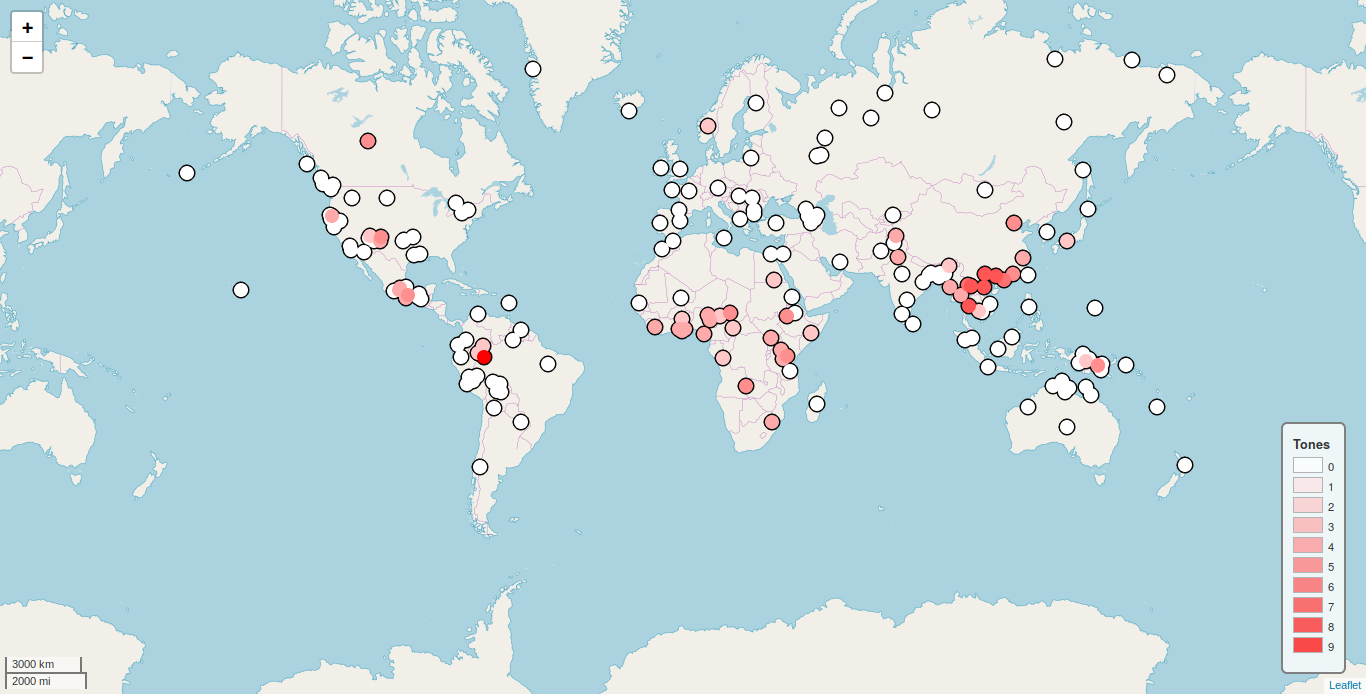
\includegraphics[width=\textwidth]{images/phoible.png}
\end{minipage}

\subsubsection{SAILS Example}

\noindent
\begin{minipage}{\textwidth}
\captionof{lstlisting}{SAILS Example}
\begin{lstlisting}
 import lingtypology
 
 #Get SAILS data for pages 'ICU3' and 'ICU4'
 sails = lingtypology.db_apis.Sails('ICU3', 'ICU4')
 df = sails.get_df()
 df.head().to_csv('tables/sails.csv')
 
 m = lingtypology.LingMap(df.language)
 m.add_features(df.ICU3_desc)
 #Use page description as legend title
 d = sails.feature_descriptions('ICU3').Description
 m.legend_title = d.at[0]
 m.start_location = (9, -79)
 m.start_zoom = 5
 m.legend_position = 'bottomleft'
 m.save_static('images/sails.png')
\end{lstlisting}
\end{minipage}

\noindent
\begin{minipage}{\textwidth}
\captionof{table}{SAILS Example}
\begin{adjustbox}{max width=\textwidth}
\begin{tabular}{ l | l | l | c | c | r | r | r }
    ~ & language & coordinates & ICU3 & ICU3\_desc & ICU4 & ICU4\_desc \\
    \hline
    0 & Baniva & (5.26123, -67.56326999999999) & 1 & Yes & 0 & No \\
    1 & Apolista & (-14.83, -68.66)" & 0 & No & ? & ? \\
    2 & Yavitero & (2.800281, -68.08421899999999) & 1 & Yes & 0 & No \\
    3 & Resígaro & (-2.48139, -71.35778) & 0 & No & 0 & No \\
    4 & Tol & (14.66859,  -87.03719) & 0 & No & 0 & No \\
\end{tabular}
\end{adjustbox}
\end{minipage}
\bigskip

\noindent
\begin{minipage}{\textwidth}
\captionof{figure}{SAILS Example}
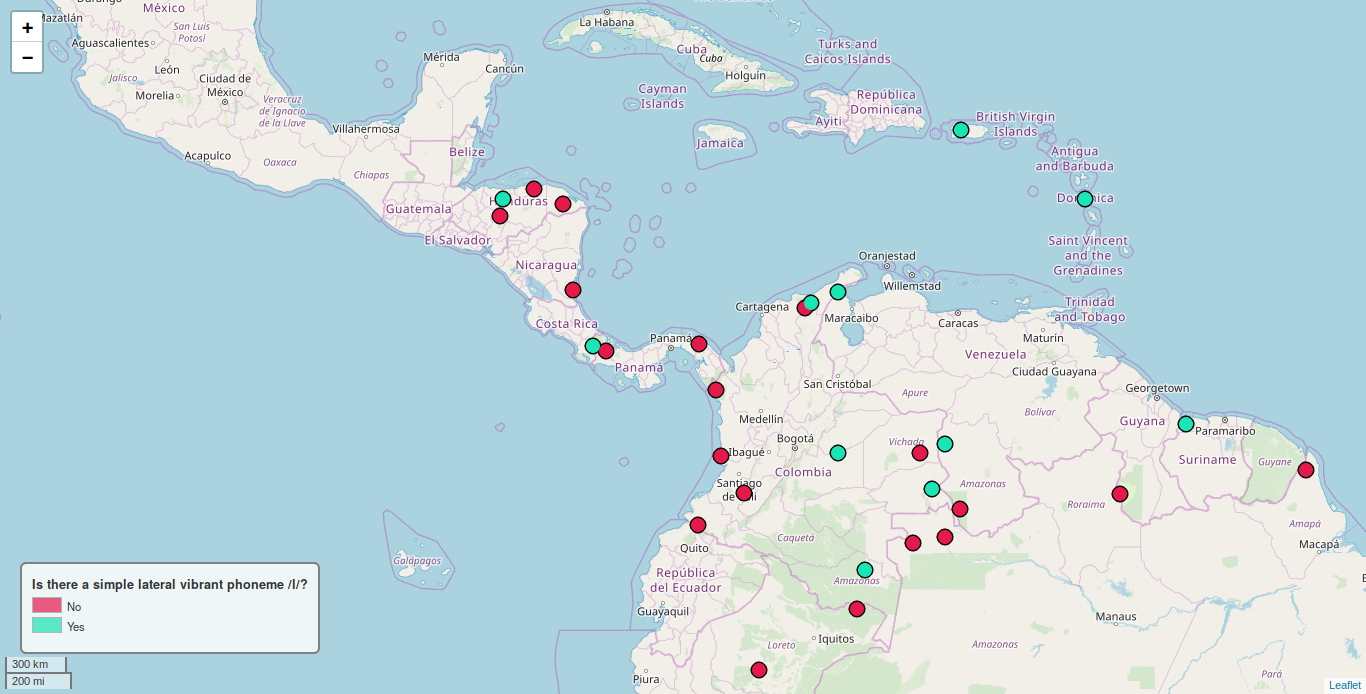
\includegraphics[width=\textwidth]{images/sails.png}
\end{minipage}

\newpage

\section{High Elevation: Ejectives}

\subsection{Introduction}

There are certain studies that suggest that geography may have influence on phonetics. For example there is a study that shows correlation between climatic areas and sonority classes~\parencite{climatesSonorants}.

Another example of such studies is article by Caleb Everett that suggests influence of elevation on ejective consonants~\parencite{ejectives}.

In this work the hypothesis that ejective consonants are more frequent in high elevation areas (higher than 1500 m) is proven for the data from the respective WALS chapter~\parencite{wals7}.

The functionality of LingTypology allows to easily check this hypothesis on all the PHOIBLE datasets. And the fact that LingTypology is open-source and is distributed under free software license guarantees reproducibility of the findings.

\subsection{Analysis}

PHOIBLE database contains the following datasets:
\begin{itemize}
 \item SAPHON: South American Phonological Inventory Database~\parencite{saphon}.
 \item AA: Alphabets of Africa~\parencite{aa}.
 \item GM: `Christopher Green and Steven Moran extracted phonological inventories from secondary sources including grammars and phonological descriptions with the goal of attaining pan-Africa coverage`~\parencite{gm}.
 \item PH: `Christopher Green and Steven Moran extracted phonological inventories from secondary sources including grammars and phonological descriptions with the goal of attaining pan-Africa coverage`~\parencite{gm}.
 \item RA: Common Linguistic Features in Indian Languages: Phoentics~\parencite{ra}.
 \item SPA: Stanford Phonology Archive~\parencite{spa}.
 \item UPSID: UCLA Phonological Segment Inventory Database~\parencite{upsid}.
\end{itemize}

In this study RA and AA are not use because they either do not contain languages with ejectives or do not provide such information.

For all the other datasets information on amount of ejectives was collected using Lingtypology.

For all the languages I used the Lingtypology function that returns elevation for a given language based on its coordinates from Glottolog.

To check the hypothesis that can be formulated like "is it true that languages higher than 1500m are more probably has ejectives", I calculated chi-square test of the distribution of languages with or without ejectives and higher or lower than 1500m.

To the hypothesis from the Everett's article I added another hypothesis: is it true that if the language is higher, the more ejectives there are. To check this hypothesis I calculated two linear regressions for each dataset: one was calculated on the whole dataset of languages, the other was calculated only for languages that has ejectives.

\subsection{Results}

Results for the PHOIBLE datasets are stored in Table 4. The firts row is the name of the dataset, the second row is the p-value of the linear regression for languages with ejectives, the third row is the p-value of the linear regression for all languages.

The code necessary to create this table is stored in the remote repository \parencite[PHOIBLE: Quantitative Research.ipynb]{lingtypologyResearch}. This code is common 
for all the work with Phoible and elevation. It uses \texttt{lingtypology}, \texttt{scipy} and \texttt{matplotlib} libraries~\parencite{scipy}~\parencite{matplotlib}.

\noindent
\begin{minipage}{\textwidth}
\captionof{table}{Ejectives. P-value Table}
\begin{adjustbox}{max width=\textwidth}
\begin{tabular}{ l | l | c | c | c }
    ~  & Dataset  & Regression (with ejectives only)  & Regression (all languages)  & Chi2 Test \\
    \hline
    0  & UPSID  & 0.95055  & 0.00004  & 0.00003 \\
    1  & SPA  & 0.47553  & 0.00001  & 0.00018 \\
    2  & PH  & 0.73152  & 0.39245  & 0.16019 \\
    3  & GM  & 0.03858  & 0.00000  & 0.00000 \\
    4  & SAPHON  & 0.018874  & 0.00000  & 0.00038 \\
    \hline
\end{tabular}
\end{adjustbox}
\end{minipage}
\bigskip

There are two possible ways to treat these numbers. The simplest option is to treat the datasets as equal and take median p-values. In this case those would be 0.47554, 0.00001 and 0.00018 for the regressions and chi-square respectively.

The second option is to treat the datasets as diffirent and consider only worldwide datasets. In this case, only UPSID and SPA will be considered.

Nevertheless, in both options the result will be the same: the second regression and chi-square test show p-value < 0.05.

This means that it is indeed true that the share of languages with ejectives is higher if the elevation is more than 1500m. This fact causes the linear regression for all languages (including the ones with no ejectives) to be statically significant. Nevertheless, \textbf{it is not true} that the higher the language, the more ejectives there are, due to the fact that the regression for the languages that has ejectives does not show statistically significant result.

To demonstrate the results on the map, I provide map with languages that has ejectives (Figure 6) for UPSID dataset. It is noticable that these languages tend to be in high elevation areas, now it is proven statistically for Phoible datasets The code used to generate it is in Appendix: Listing 3.

\noindent
\begin{minipage}{\textwidth}
\captionof{figure}{Languages with Ejectives}
\includegraphics[width=\textwidth]{images/picture6.png}
\end{minipage}

\subsection{Discussion}

Of course, "correlation does not imply causation", and at the moment it is impossible to claim cause-and-effect relation for high elevation and presence of ejective consonants. Certain studies speculate why there may be cause-and-effect relations for geographical properties of regions and phonetics (e.g. \parencite{ejectives} and \parencite{climatesSonorants}. Nevertheless, it seems that further research is needed. LingTypology provides functionality that could be used in such studies.

\newpage

\section{High Elevation: Quantitative Research}

\subsection{Introduction}
Lingtypology allows accessing multiple features from linguistic databases. Therefore, I decided to find out whether high elevation may define distribution of other features from PHOIBLE database.

There seems to be no scientific research on correlation of elevation and morhological or synthactic features. Nevertheless, I decided to add morphosyntactic features from Aytotyp database.

It is important to say, that such calculations in many cases do not lead to a positive result. LingTypology allows to perform such studies automatically. Therefore, time costs for such research is minimal.

\subsection{PHOIBLE}

To test this idea on PHOIBLE data I take all the phoneme properties and test them as binary. So, in this part I ask questions like: "Is it true that if elevation is higher than 1500m, then the more likely it is to meet a language that has phonemes with the property?" I use chi-square test, then I find median p-value for all the datasets.

The result is in Table 5. \textit{NaN} means that there are no languages where at least on phoneme has the given property. \textit{nan} means that there is not enough data to calculate chi-square.

As you can see, despite the fact that for certain datasets there are some p-values below 0.05, there are no phoneme properties where median p-value is below 0.05. So, there is \textbf{no} statistically significant difference in distributions of languages having phonemes with a particular property below or higher than 1500m for all the binary properties for all the PHOIBLE datasets.

\noindent
\begin{minipage}{\textwidth}
\captionof{table}{PHOIBLE All}
\begin{adjustbox}{max width=\textwidth}
\begin{tabular}{ | l | c | c | c | c | c | c |}
    \toprule
    Dataset &     short &      long & delayedRelease &       tap &     trill &     nasal \\
    \midrule
    UPSID &    0.7304 &    0.6205 &         0.6106 &    0.9272 &    0.5174 &    0.7388 \\
    SPA &    0.4974 &    0.8311 &         0.4335 &    0.9873 &    0.9605 &       nan \\
    GM &    0.6587 &    0.0070 &         0.8435 &    0.8367 &    0.9499 &    0.1603 \\
    RA &    0.0826 &    0.1125 &            nan &    0.1125 &    0.0622 &       nan \\
    AA &       NaN &    0.7559 &            nan &    0.9076 &    0.4865 &       nan \\
    PH &       NaN &    0.2549 &         0.9051 &    0.7908 &    0.1327 &    0.7573 \\
    SAPHON &       NaN &    0.0287 &         0.4856 &    0.3496 &    0.8520 &    0.7113 \\
    Median &  0.578074 &  0.254949 &       0.610642 &  0.836724 &  0.517375 &  0.725022 \\
    \bottomrule
    \toprule
    Dataset &   lateral &    labial &     round & labiodental & distributed & strident \\
    \midrule
    UPSID &    0.1174 &       nan &    0.2667 &      0.8925 &      0.8872 &   0.5576 \\
    SPA &    0.5463 &    0.3787 &    0.3787 &      0.1592 &      0.2771 &   0.7159 \\
    GM &    0.6415 &       nan &    0.1603 &      0.5869 &      0.4575 &   0.3861 \\
    RA &    0.9301 &       nan &       nan &      0.9249 &         nan &   0.3215 \\
    AA &    0.0491 &       nan &       nan &      0.1428 &      0.8365 &      nan \\
    PH &    0.3205 &       nan &       nan &      0.8006 &      0.0753 &   0.4896 \\
    SAPHON &    0.0000 &       nan &       nan &      0.8457 &      0.0139 &   0.3705 \\
    Median &  0.320519 &  0.378695 &  0.266709 &    0.800579 &    0.367317 &  0.43784 \\
    \bottomrule
    \toprule
    Dataset &       low &     front &      back &     tense & retractedTongueRoot & advancedTongueRoot \\
    \midrule
    UPSID &    0.2667 &       nan &       nan &    0.2667 &              0.1243 &                NaN \\
    SPA &    0.3787 &       nan &       nan &       nan &              0.8936 &             0.3787 \\
    GM &    0.4430 &    0.1603 &    0.1603 &    0.1603 &              0.8242 &                NaN \\
    RA &    0.3215 &       nan &       nan &       nan &              0.9301 &                NaN \\
    AA &       nan &       nan &       nan &       nan &              0.2252 &                NaN \\
    PH &    0.5906 &       nan &       nan &    0.2552 &              0.8665 &             0.2552 \\
    SAPHON &       nan &       nan &       nan &       nan &                 NaN &             0.1864 \\
    Median &  0.378695 &  0.160319 &  0.160319 &  0.255246 &            0.845344 &           0.255246 \\
    \bottomrule
    \toprule
    Dataset & epilaryngealSource & spreadGlottis & constrictedGlottis &    fortis & loweredLarynxImplosive &     click \\
    \midrule
    UPSID &                NaN &        0.3624 &             0.1280 &       NaN &                 0.5654 &       NaN \\
    SPA &                NaN &        0.8858 &             0.1328 &    0.8083 &                 0.8776 &       NaN \\
    GM &             0.1603 &        0.0480 &             0.0057 &       NaN &                 0.2245 &    0.1603 \\
    RA &                NaN &        0.8941 &             0.1244 &       NaN &                 0.3215 &       NaN \\
    AA &                NaN &        0.1302 &             0.6491 &       NaN &                 0.5679 &       NaN \\
    PH &             0.2552 &        0.8090 &             0.1432 &       NaN &                 0.9455 &       NaN \\
    SAPHON &                NaN &        0.0090 &             0.3423 &       NaN &                 0.6432 &       NaN \\
    Median &           0.207783 &      0.362376 &           0.132809 &  0.808315 &               0.567919 &  0.160319 \\
    \bottomrule
\end{tabular}
\end{adjustbox}
\end{minipage}
\bigskip

\subsection{Autotyp}

Also, I checked this idea for numeric features from Autotyp. In this case linear regression was used.

All calculations are performed by the code from the remote repository~\parencite[PHOIBLE: Quantitative Research.ipynb]{lingtypologyResearch}. This code uses LingTypology and SciPy~\parencite{scipy}.

Among the 30 numeric features there were 4 features that showed p-value < 0.05.
These features are represented in Table 6. In this table the features are represented as abbreviations that are not always clear. Therefore I provide the list of descriptions for features from the Autotyp repository~\parencite[metadata\_overview.csv]{autotyp}:
\begin{itemize}
 \item `Exponence: number of categories that are expressed in the same marker`.
 \item `Rough approximation of the size of the possessum category in terms of the number of semantic classes covered`.
 \item `Number of separately marked inflectional categories (including agreement) in position "post" of the verb`.
 \item `Number of morpheme types included in a phonologically or grammatically coherent suffix domain`.
\end{itemize}

\noindent
\begin{minipage}{\textwidth}
\captionof{table}{Autotyp Features}
\begin{tabular}{lll}
\toprule
Feature &                    Subfeature &     P-value \\
\midrule
Grammatical\_markers &                   Exponence.n &  0.00000000 \\
NP\_structure &          NPHeadSemClassSize.n &  0.01766784 \\
VInfl\_counts\_per\_position &          VInflCatAndAgrPost.n &  0.02895302 \\
Word\_domains &  MphmTypesInCohSuffixDomain.n &  0.00196901 \\
\bottomrule
\end{tabular}
\end{minipage}
\bigskip

\subsection{Discussion}

So, in the case of PHOIBLE features the result is negative: no statistically significant differences were found in distribution of languages having phonemes with certain characteristics and high elevation.

In the case of Autotyp there were found several linear regressions with p-value < 0.05. However, I did not find any papers mentioning influence of geography on morphosynthax. Therefore, it is secure to say that futher research is needed.

LingTypology provides easy means to reproduce my research on Phoible and Autotyp and expand it.
\newpage

\section{WALS: Quantitative Research}

Sometimes it is interesting to try to find correlations that does not have any theoretical background. Doing it manually is very inefficient because of the time costs. LingTypology suggests a way to simplify such studies. It is possible to get multiple features from different online databases. This allows to prepare data for a study very easily and then perform statistical calculations for it.

To demonstrate it, I used LingTypology to get all the WALS pages that has binary features (e.g. something is present in a language or not present) and calculated chi-square tests for each pair of pages. There are 17 binary features in WALS. So, 289 p-values were calculated.

It was done to find out whether there are implicative universaliae or frequentaliae connecting the language features from these WALS pages.

The full code of the program is mostly general (calculating chi-square, assembling the matrix etc.). I include the part that uses lingtypology into the listing below. This code gets all features from the WALS database. The full code is stored in the remote repository \parencite[WALS: Quantitative Research.ipynb]{lingtypologyResearch}.
\bigskip

\noindent
\begin{minipage}{\textwidth}
\captionof{lstlisting}{WALS: All Features}
\begin{lstlisting}
 from lingtypology.db_apis import Wals
 features_list = Wals().features_list
 w = Wals(*features_list)
 data = w.get_df(join_how='outer')
\end{lstlisting}
\end{minipage}
\bigskip

The result of such calculations is matrix where headers and indexes are names of WALS features and values are p-values. This matrix is too large to be included into the text, so it is stored in the remote repository~\parencite[WALS: Quantitative Research.ipynb]{lingtypologyResearch}. For convenience, I include small part of it in the table below. \texttt{nan} means that there was not enough data to calculate chi-square (e.g. no common languages for the given pair of pages).

No p-values below 0.05 were found. Therefore, the result of this study is negative. This result is the expected one because none of the tested features are known to correlate.

\noindent
\begin{minipage}{\textwidth}
\captionof{table}{WALS Matrix}
\begin{tabular}{|l|cccc|l|}
\hline
feature & \_10A\_desc & \_25B\_desc & \_39B\_desc & \_47A\_desc & ... \\
\hline
\_10A\_desc &   1.00000 &   0.99444 &       nan &   0.63296 &   ... \\
\_25B\_desc &   0.90442 &   1.00000 &       nan &   0.96609 &   ... \\
\_39B\_desc &   1.00000 &       nan &   1.00000 &   0.66501 &   ... \\
\_47A\_desc &   0.82120 &   0.84267 &   0.66501 &   1.00000 &   ... \\
\hline
... &   ... &   ... &       ... &   ... &   ... \\
\hline
\end{tabular}
\end{minipage}

\newpage

\section{Conclusion}

Python programming language is widely used by linguists. In this thesis I have presented a new package for linguistic typology: LingTypology. It allows to access multiple online linguistic databases and create linguistic interactive maps.

Both features of the package may be of use for typological studies.

Databases API increases productivity of typological research allowing researchers to access massive amount of data automatically. Also, it simplifies reproduction of linguistic studies.

To demonstrate the functionality of LingTypology, I included several typological studies made with the package.

The first research reproduces some conclusions of Everett's article~\parencite{ejectives} on the data from the PHOIBLE datasets and reaches the same conclusion: share of languages with ejective consonants is higher in high elevation areas.

Also, I performed two small quantitative studies on PHOIBLE, Autotyp and WALS databases to demonstrate the ease of finding correlations that do not have a theoretical background with LingTypology.

In the first study, I try to find a correlation with other PHOIBLE features and elevation and Autotyp features and elevation. In the case of PHOIBLE I used chi-square statistical test and in the case of Autotyp I used linear regression. On PHOIBLE data the result was negative while on Autotyp data some regressions had p-value < 0.05. In Autotyp there were several linear regressions that showed p-value < 0.05.

In the second study I search for implicative universaliae in WALS. To gain the result I check all pairs of binary features from WALS and calculate chi-square test for each pair. The result is negative.

The second feature of LingTypology -- interactive maps -- can be useful for visualization of typological research. LingTypology package allows to draw linguistic maps with Glottolog data at its core~\parencite{HaraldHammarstrom2019}.

The map could be rendered as HTML which is useful for implementing it into websites and including into web-publications. The other option is to freeze the map as PNG. It allows to include it into handouts and papers.

By default the maps generated are colored. However, LingTypology allows to create black and white maps because some journals does not support color printing.

LingTypology is a well-documented package. The full reference manual is included into Chapter 3 of this thesis. Full technical documentaion may be found in the docstrings. The repository of the package contain a full tutorial for LingTypology~\parencite{Govnov2019}.

In the future I plan to add more linguistic databases (e.g. ABVD \parencite{abvd}) so that the package could be find useful in wider range of scientific research.

Also, I plan to add density contourplot to the linguistic maps using kernel density estimation algorithm (more abou KDE here \parencite{kde}). It would allow to create isogloss automatically.

\newpage

\section{References}
\printbibliography[type=misc, title=Programming Tools]
\printbibliography[type=manual, title=Documentation]
\printbibliography[type=online, title=Online Recources]
\printbibliography[type=article, title=Articles]
\defbibfilter{other}{
  type=book or
  type=incollection
}
\printbibliography[filter=other, title=Other]
\newpage
\section{Appendix}

\textbf{Listing 1. Wals 1A map with default Lingtypology strokes.}
\begin{lstlisting}
import os
os.chdir('images')
import lingtypology

wals_page = lingtypology.db_apis.Wals('1a', '2a').get_df()
m = lingtypology.LingMap(wals_page.language)
m.add_custom_coordinates(wals_page.coordinates)
m.add_features(wals_page._1A)
m.legend_title = 'Consonant Inventory'
m.colors = lingtypology.gradient(5, 'yellow', 'green')
m.save_static('LingtypologyStrokeAppearance.png')
\end{lstlisting}
\bigskip

\textbf{Listing 2. Wals 1A map with default Folium strokes.}
\begin{lstlisting}
import os
os.chdir('images')
import lingtypology

wals_page = lingtypology.db_apis.Wals('1a', '2a').get_df()
m = lingtypology.LingMap(wals_page.language)
m.add_custom_coordinates(wals_page.coordinates)
m.add_features(wals_page._1A)
m.legend_title = 'Consonant Inventory'
m.colors = lingtypology.gradient(5, 'yellow', 'green')
m.unstroked = False
m.save_static('FoliumStrokeAppearance.png')
\end{lstlisting}
\bigskip

\textbf{Listing 3. Languages with Ejectives.}
\begin{lstlisting}
import lingtypology

df = lingtypology.db_apis.Phoible(subset='UPSID', aggregated=False).get_df()
#Get all languages with ejectives
df = df[df.raisedLarynxEjective == '+']
#Remove duplicates
df = df.drop_duplicates(subset='Glottocode')

m = lingtypology.LingMap(df.Glottocode, glottocode=True)
#Tiles with terrain
m.tiles = 'Stamen Terrain'
m.title = 'Languages with Ejectives'
m.radius = 5
m.opacity = 0.5
m.colors = ('blue',)
m.save_static('images/Picture6.png')
\end{lstlisting}

\end{document} 
